% Load essential packages
\usepackage{lipsum}          % Dummy text
\usepackage[utf8]{inputenc}  % Input encoding
\usepackage[T1]{fontenc}     % Font encoding
\usepackage[english]{babel}  % Language settings
\usepackage{lmodern}         % Modern LaTeX fonts
\usepackage{layout}          % Layout customization

% Using biblatex with IEEE style
\usepackage{csquotes}
\usepackage{scrhack}
\usepackage[backend=biber, style=numeric, sorting=none, maxbibnames=6, minbibnames=1]{biblatex}
\addbibresource{bibliography.bib}  % Link to your BibTeX database file

\usepackage{calc}


% Mathematical symbols and environments
\usepackage{amsmath, amsfonts, amssymb, mathrsfs}

\usepackage{changepage}

% Do not include the chapter in numbering
\usepackage{chngcntr}
\counterwithout{equation}{chapter}  % Detach equation counter from chapter
\counterwithout{figure}{chapter}    % Detach figure counter from chapter
\counterwithout{table}{chapter}     % Detach table counter from chapter

% Algorithms
\usepackage{algorithm}
\usepackage[table,xcdraw]{xcolor}
\usepackage[hang,flushmargin]{footmisc} 
\usepackage{booktabs}
\usepackage{bm,bbm}
\usepackage[noend]{algpseudocode}
\newcommand\Algphase[1]{%
\vspace*{-0.5\baselineskip}\Statex\hspace*{\dimexpr-\algorithmicindent-2pt\relax}\rule{0.9\textwidth}{0.4pt}%
\Statex\hspace*{-\algorithmicindent}\textbf{#1}%
\vspace*{-0.5\baselineskip}\Statex\hspace*{\dimexpr-\algorithmicindent-2pt\relax}\rule{0.9\textwidth}{0.4pt}%
}

\usepackage{multirow}
\usepackage{arydshln} % this causes problems with the superborder glossary style formatting
\dashlinegap=2pt

\usepackage{colortbl}
\usepackage{adjustbox}

% Graphics, figures, and subcaptions
\usepackage{graphicx}
\graphicspath{{img/}}        % Root directory for graphics
\usepackage{subcaption}      % Subfigures
\usepackage{float}           % Better float control
\usepackage{placeins}        % use \FloatBarrier to prevent floats (figures, tables, ...) from passing a specific point such as start of the next section
\usepackage{wrapfig}         % Wrapping text around figures

% PDF handling
\usepackage{pdfpages}

% caption formatting
\usepackage{caption}
\DeclareCaptionLabelSeparator{colon}{: }
\captionsetup{
    format=plain, % alignes multiline caption text with "Figure", "Table", etc. rather than with the beginning of the caption text
    %format=hang, % alignes multiline caption text with the beginning of the caption text
    labelsep=colon,
    labelformat=simple
}


% Header/footer customization
\usepackage[headsepline, footsepline, plainfootsepline]{scrlayer-scrpage}
\clearpairofpagestyles
\automark{chapter}
\ihead{\leftmark{}}
\ofoot[\thepage]{\thepage}



% Indentation and spacing
\setlength{\parindent}{0cm}  % No indentation at the beginning of paragraphs
\setlength{\parskip}{1em}    % Adjust space between paragraphs

% Notes and annotations
\usepackage[ngerman,linecolor=gray,bordercolor=gray,backgroundcolor=yellow]{todonotes}

% Code highlighting
\usepackage{listings}
\usepackage{color}
\definecolor{mygreen}{rgb}{0,0.6,0}
\definecolor{mymauve}{rgb}{0.58,0,0.82}
\lstset{
  basicstyle=\ttfamily,
  breaklines=true,
  captionpos=b,
  commentstyle=\color{mygreen},
  escapeinside={\%*}{*)},
  keywordstyle=\color{blue},
  stringstyle=\color{mymauve},
  frame=single,
  frameround=tttt
}

% Title, author, and date settings
\title{Prosodic Feature Modelling in Transformers for Speaker Verification}
\author{Fabian Bosshard, Andrin Fassbind}
\date{\today}
\makeatletter
\let\myTitle\@title
\makeatother

% Hyperlink settings
\usepackage[hidelinks, pdftex]{hyperref}
\hypersetup{
  pdftitle={\myTitle},
  pdfdisplaydoctitle=true,
  bookmarksnumbered,
  pdfstartview={FitH}
}

% Enumerated lists customization
\usepackage{enumitem}

% Diagrams and plots
% \usepackage{pgfplots, pgfplotstable, sfmath} %sfmath verändert die Schriftart in Formeln
\usepackage{pgfplots, pgfplotstable}
\pgfplotsset{compat=1.18} % adjust to your version
\usetikzlibrary{patterns, arrows, shapes, positioning, arrows.meta, calc, math, 3d, matrix}


% lengths

\newlength{\melwidth}
\newlength{\melheight}

\newlength{\imageheight}
\settoheight{\imageheight}{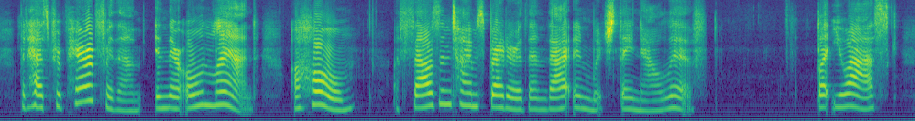
\includegraphics{spectrogram.pdf}}

\newlength{\imagewidth}
\settowidth{\imagewidth}{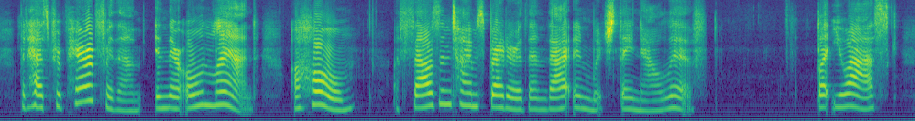
\includegraphics{spectrogram.pdf}}

\newlength{\halfimagewidth}
\setlength{\halfimagewidth}{0.5\imagewidth}





% Text formatting for bibliography
\usepackage{ragged2e}

% Acronym handling
\usepackage[nopostdot, nogroupskip, style=super, nonumberlist]{glossaries}
\setlength{\glsdescwidth}{0.8\textwidth}
\makeglossaries

\newacronym{ai}{AI}{artificial intelligence}
\newacronym{lm}{LM}{language model}
\newacronym{llm}{LLM}{large language model}
\newacronym{gpt}{GPT}{Generative Pre-trained Transformer}
\newacronym{rl}{RL}{reinforcement learning}
\newacronym{ml}{ML}{machine learning}
\newacronym{nlp}{NLP}{natural language processing}
\newacronym{xai}{XAI}{explainable artificial intelligence}
\newacronym{hmi}{HMI}{human-machine interaction}
\newacronym{sota}{SOTA}{state-of-the-art}
\newacronym{zhaw}{ZHAW}{Zurich University of Applied Sciences}

\newacronym{mlp}{MLP}{multilayer perceptron}
\newacronym{dnn}{DNN}{deep neural network}
\newacronym{cnn}{CNN}{convolutional neural network}
\newacronym{rnn}{RNN}{recurrent neural network}
\newacronym{lstm}{LSTM}{long short term memory}
\newacronym{blstm}{BLSTM}{bidirectional long short-term memory}
\newacronym{hmm}{HMM}{hidden Markov model}
\newacronym{gan}{GAN}{generative adversarial network}
\newacronym{resnet}{ResNet}{residual neural network}
\newacronym{ssast}{SSAST}{self-supervised audio spectrogram transformer}
\newacronym{vit}{ViT}{Vision Transformer}

\newacronym{sr}{SR}{speaker recognition}
\newacronym{sv}{SV}{speaker verification}
\newacronym{si}{SI}{speaker identification}
\newacronym{sc}{SC}{speaker clustering}
\newacronym{asr}{ASR}{automatic speech recognition}
\newacronym{far}{FAR}{false acceptance rate}
\newacronym{frr}{FRR}{false rejection rate}
\newacronym{eer}{EER}{equal error rate}
\newacronym{cer}{CER}{character error rate}
\newacronym{wer}{WER}{word error rate}
\newacronym{mr}{MR}{misclassification rate}
\newacronym{rer}{RER}{relative error rate}
\newacronym{mse}{MSE}{mean squared error}
\newacronym{infonce}{InfoNCE}{information noise-contrastive estimation}
\newacronym{adam}{Adam}{adaptive moment estimation}

\newacronym{fft}{FFT}{fast Fourier transform}
\newacronym{stft}{STFT}{short-time Fourier transform}
\newacronym{mfcc}{MFCC}{mel-frequency cepstral coefficient}
\newacronym{snr}{SNR}{signal-to-noise ratio}
\newacronym{sst}{SST}{supra-segmental temporal information}
\newacronym{fba}{FBA}{frame-based acoustic information}
\newacronym{os}{OS}{original segment}
\newacronym{ss}{SS}{shuffled within segment}
\newacronym{su}{SU}{shuffled within utterance}

\newacronym{ctc}{CTC}{connectionist temporal classification}
\newacronym{lpc}{LPC}{linear predictive coding}
\newacronym{cpc}{CPC}{contrastive predictive coding}
\newacronym{apc}{APC}{autoregressive predictive coding}
\newacronym{mhsa}{MHSA}{multi-head self-attention}

\newacronym{mo}{$\mathcal{M}_\text{o}$}{model pretrained on original spectrograms}
\newacronym{ms}{$\mathcal{M}_\text{s}$}{model pretrained on shuffled spectrograms}
\newacronym{moo}{$\mathcal{M}_\text{o/o}$}{model pretrained on original and finetuned on original spectrograms}
\newacronym{mos}{$\mathcal{M}_\text{o/s}$}{model pretrained on original and finetuned on shuffled spectrograms}
\newacronym{mso}{$\mathcal{M}_\text{s/o}$}{model pretrained on shuffled and finetuned on original spectrograms}
\newacronym{mss}{$\mathcal{M}_\text{s/s}$}{model pretrained on shuffled and finetuned on shuffled spectrograms}
